\documentclass[conference]{IEEEtran}

\usepackage{cite}
\usepackage{amsmath,amssymb,amsfonts}
\usepackage{algorithmic}
\usepackage{graphicx}
\usepackage{textcomp}
\usepackage{xcolor}
\usepackage{subfigure}

% Tweaking the math symbols library
\DeclareMathOperator\atanh{atanh}

\begin{document}

\title{CORTEZ1 - A 130nm Skywater-designed\\ASIC for character recognition}

\author{\IEEEauthorblockN{Simone Corbetta}
simone.corbetta@gmail.com}

\maketitle

\begin{abstract}
\end{abstract}

\begin{IEEEkeywords}
\end{IEEEkeywords}

\section{Introduction}\label{sec:intro}



\section{Network architecture}\label{sec:nnet}
\subsection{Input problem}\label{ssec:boulder}
The input vector consists of a $5x5$ grid of bipolar values. The network is capable of classifying
input grids representing the $5$ vowels of the English alphabet, as shown in Figure
\ref{fig:charsIn}.

\begin{figure*}
    \centering
    \subfigure[Vowel A]{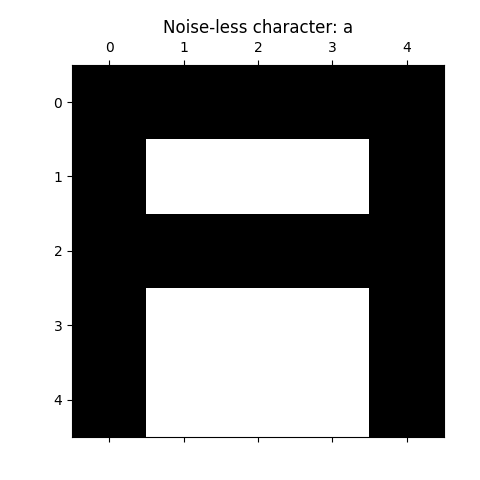
\includegraphics[width=0.18\textwidth]{images/vanilla_a.png}}
    \subfigure[Vowel E]{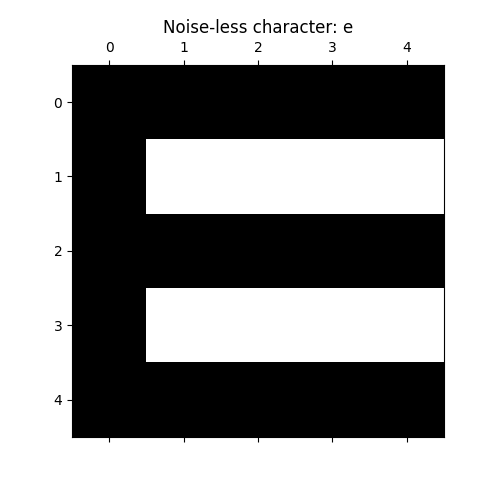
\includegraphics[width=0.18\textwidth]{images/vanilla_e.png}}
    \subfigure[Vowel I]{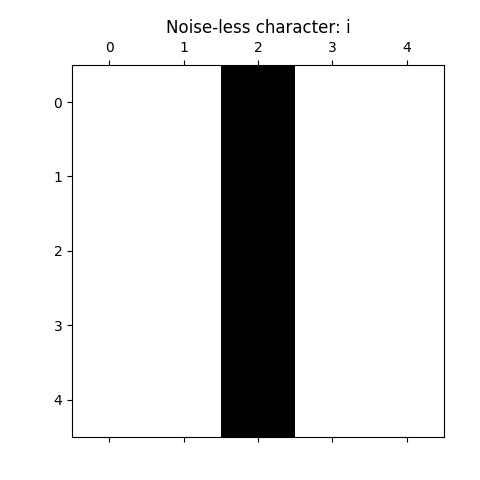
\includegraphics[width=0.18\textwidth]{images/vanilla_i.png}}
    \subfigure[Vowel O]{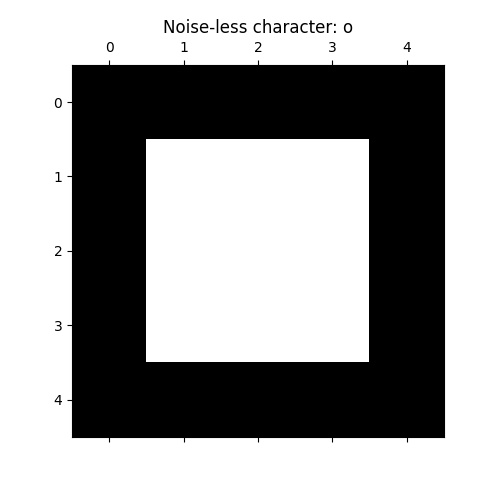
\includegraphics[width=0.18\textwidth]{images/vanilla_o.png}}
    \subfigure[Vowel U]{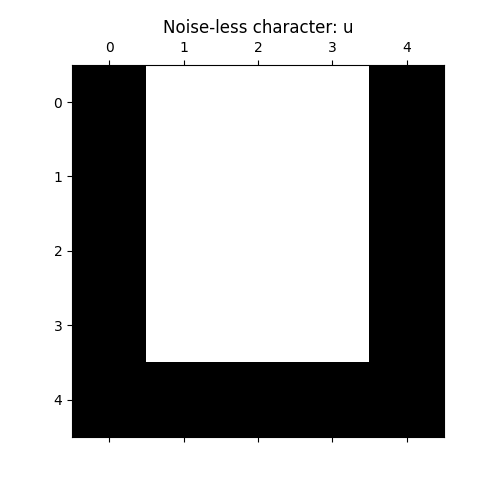
\includegraphics[width=0.18\textwidth]{images/vanilla_u.png}}
    \label{fig:charsIn}
    \caption{Input problem and recognizable vowels}
\end{figure*}

\begin{figure*}
    \centering
    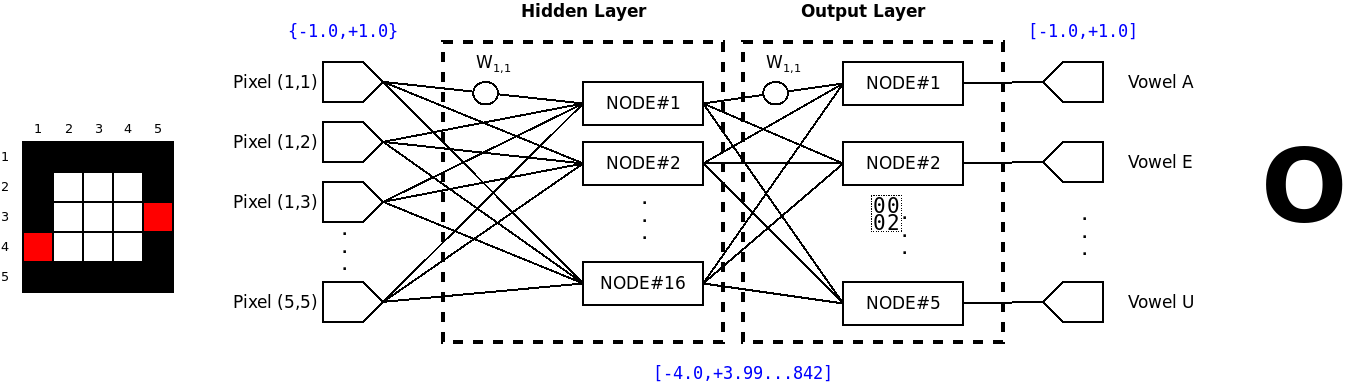
\includegraphics[width=\textwidth]{images/Architecture.png}
    \label{fig:netArchi}
    \caption{Architecture of the Neural Network}
\end{figure*}
The architecture of the designed Neural Network is shown in Figure \ref{fig:netArchi}. At the
highest level the network behaves as a Madaline network \cite{23872}, in that inputs and outputs
take bipolar values in the ${-1.0, 1.0}$ set. However, the internals of the network work with
fractional values, i.e. fixed-point values bounded to the $[-1.0,1.0]$ range.

The network is composed of two layers. An Input Layer connects $25$ inputs to $16$ neurons. An
Output Layer connects $16$ neurons to $5$ output nodes. Pixels from the $5x5$ input grid are all
mapped to inputs, while the output vector encodes the prediction as one-hot. Input and Output layer
are both fully connected.

recognized. All $25$ pixels take values in the ${-1.0,1.0}$ set, corresponding to the white
respectively dark pixels in the image. Up to $3$ noisy pixels are covered. A noisy pixel (shown in
red in Figure \ref{fig:netArchi}) is one that inverts its value from the original specification
found in Figure \ref{fig:charsIn}.


\section{Design}\label{sec:design}
\begin{figure}
    \centering
    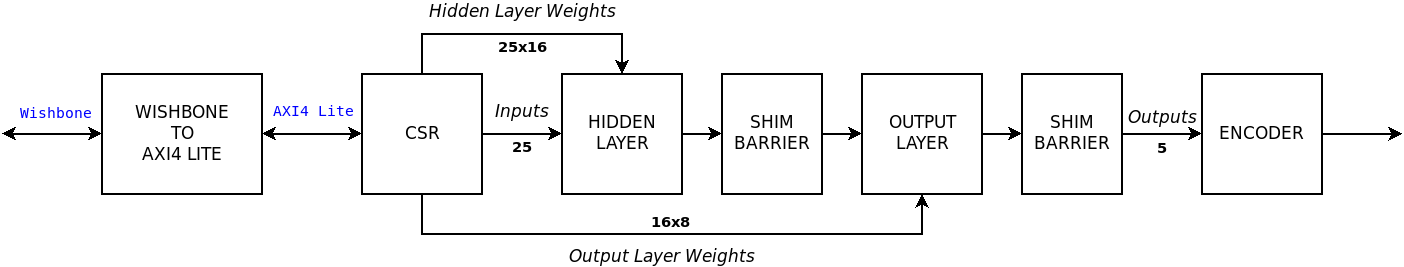
\includegraphics[width=0.95\columnwidth]{images/BlockDiagram.png}
    \label{fig:bd}
    \caption{Design core block diagram}
\end{figure}

Figure \ref{fig:bd} shows the design core's block diagram. The top-level interface consists of a
simple single-cycle Write/Read Wishbone interface and the primary binary output solution. The
Wishbone interface and the primary outputs are then harnessed within Caravel.

The neural network is implemented by the central blocks: the \texttt{HIDDEN LAYER} and the
\texttt{OUTPUT LAYER}. Weights are stored in a volatile register pool within the \texttt{CSR} block.
Their values are fixed for a particular recognition problem, but they can be updated for different
problems that the same architecture caould solve. Inputs are forced through Software-controlled
registers. A control register is used to trigger the first layer of the network. A status register
can then be polled while waiting for the solution to exist. The last block, the \texttt{ENCODER}, is
used to encode the solution found by the network so that it can be used at the higher levels of the
SoC. In our case, the encoded output consists of enable signals for a 7-segments LED display that
will show the classified vowel. Since neurons in each layer can fire any time, depending on the
inputs and the weights, a \texttt{SHIM BARRIER} is used to align them before presenting to the
downstream logic.

\subsection{Activation function}\label{ssec:actFun}
The chosen activation function, $\tanh$, maps values from $\mathbb{R}$ to $[-1.0,1.0] \subset
\mathbb{R}$. However, few approximations can be tailored to simplify the design of the circuit.

At first it is easy to verify that the $\tanh$ function is odd symmetrical. The computational problem
can then be reduced by half the size: absolute value is taken for any input, and the function is
evaluated only for the $[0,\infty)$ range only. Later in the circuit, negative values are re-signed
when appropriate by a simple change of sign.

The half function is the approximated to a piecewise linear function. As a matter of fact, the
$\tanh$ function has some interesting properties: \textit{1)} for small angles, $\tanh(x)$ can be
approximated to $x$ and \textit{2)} for larger values there is a plateau around $2.0$. The proposed
piecewise linear approximation consists of 4 (four) different segments:

\begin{equation}
    y = 
        \begin{cases}
            f_{1}^{pw}(x) & x \in [0,\atanh(\sqrt{1/3})] \\
            f_{2}^{pw}(x) & x \in [\atanh(\sqrt{1/3}),\atanh(\sqrt{2/3})] \\
            f_{3}^{pw}(x) & x \in [\atanh(\sqrt{2/3}),2] \\
            f_{4}^{pw}(x) & x \geq 2
        \end{cases}
\end{equation}

\begin{table}
    \centering
    \label{tab:pwParams}
    \caption{Linear parameters of piecewise segments}
    \begin{tabular}{|c|c|c|} \hline
        \textbf{SEGMENT} & \texttt{m} & \texttt{q} \\ \hline
        $f_{1}^{pw}(x)$ & 0.8768 & 0 \\ \hline
        $f_{2}^{pw}(x)$ & 0.4903 & 0.2545 \\ \hline
        $f_{3}^{pw}(x)$ & 0.2149 & 0.5702 \\ \hline
        $f_{4}^{pw}(x)$ & 0 & 1 \\ \hline
    \end{tabular}
\end{table}
Each segment is a linear function in the form $y = mx + q$ whose parameters are specified in Table
\ref{tab:pwParams}.

\begin{figure}
    \centering
    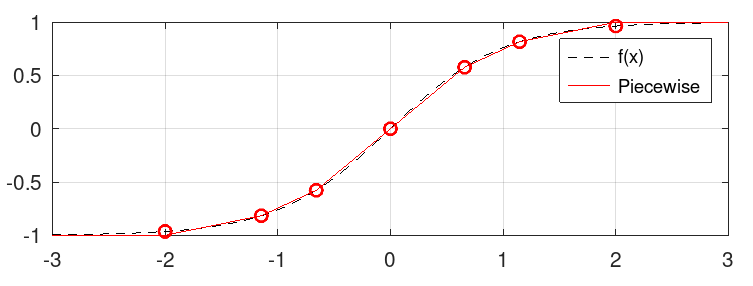
\includegraphics[width=0.95\columnwidth]{images/tanhPW.png}
    \label{fig:tanhPW}
    \caption{Piecewise approximation of the $\tanh$ function}
\end{figure}
The piecewise approximation of the desired $\tanh$ function is shown in Figure \ref{fig:tanhPW}. It
has been shown that the estimate error across the reference $[-4.0,+4.0)$ range evaluates at ????.

\begin{figure}
    \centering
    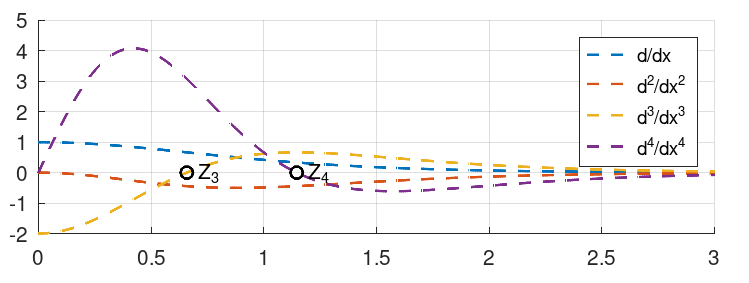
\includegraphics[width=0.95\columnwidth]{images/tanhDerivatives.png}
    \label{fig:tanhDiffs}
    \caption{$\tanh$ and its derivatives}
\end{figure}
Switch points in the piecewise function are chosen by close inspection of the $\tanh$ function and
its derivatives. Figure \ref{fig:tanhDiffs} depicts the first through fourth derivative of the
function.

The lower bound $0$ of the $f_{1}^{pw}$ segment comes from the symmetry of $\tanh$; the upper bound
$Z_{3} = \atanh(\sqrt{1/3})$ is the point where $d^{3}/dx^{3} = 0$. This is the point where the
$d/dx$ changes convexity. Same reasoning applies to the upper bound of $f_{2}^{pw}$, where $Z_{4} =
\atanh(\sqrt{2/3})$, i.e. when $d^{4}/dx^{4} = 0$. Last, $x = 2$ is an interesting point since a
plateau starts to appear. This is visible by noticing that all derivatives tend to $0$ at that
point.


\section{Tapeout}\label{sec:asic}

\section{Characterization}\label{sec:results}

\section{Conclusions}

\bibliographystyle{IEEEtran}
\bibliography{CORTEZ1}

\end{document}
